% !TEX encoding = UTF-8 Unicode
% $Header: /cvsroot/latex-beamer/latex-beamer/solutions/conference-talks/conference-ornate-20min.en.tex,v 1.6 2004/10/07 20:53:08 tantau Exp $

\documentclass{beamer}

% This file is a solution template for:

% - Talk at a conference/colloquium.
% - Talk length is about 20min.
% - Style is ornate.

\mode<presentation>
{
  \usetheme{Warsaw}
  % or ...

  \setbeamercovered{transparent}
  % or whatever (possibly just delete it)
  
  \setbeamertemplate{navigation symbols}{}
  
  \newcommand*\oldmacro{}%
  \let\oldmacro\insertshorttitle%
  \renewcommand*\insertshorttitle{%
    \oldmacro\hfill%
    \insertframenumber\,/\,\inserttotalframenumber}
}

\usepackage[utf8]{inputenc}
% or whatever

\usepackage{times}
\usepackage{multirow}
\usepackage[T1]{fontenc}
\usepackage[french]{babel}
\usepackage{graphicx}
\usepackage{eso-pic}
\usepackage{color}
\usepackage{tikz}
\usepackage{wasysym}

% Or whatever. Note that the encoding and the font should match. If T1
% does not look nice, try deleting the line with the fontenc.

%\title[Tours de magie]
%{}

%\titlegraphic{\raisebox{2em}{}}

\author[Prologin]
{\includegraphics{prologin2014}}

\date
{}

\begin{document}

\definecolor{vert}{rgb}{0.07 0.54 0.07}

%\section{Intervenants}

\begin{frame}
%	\frametitle{PUROGURAMU}
	\vspace{0.5cm} \centering \includegraphics[width=0.9\linewidth]{prologin2014}
\end{frame}

%\subsection{MOOC en Inde}

\begin{frame}
	\frametitle{Jeu à 4 joueurs}
	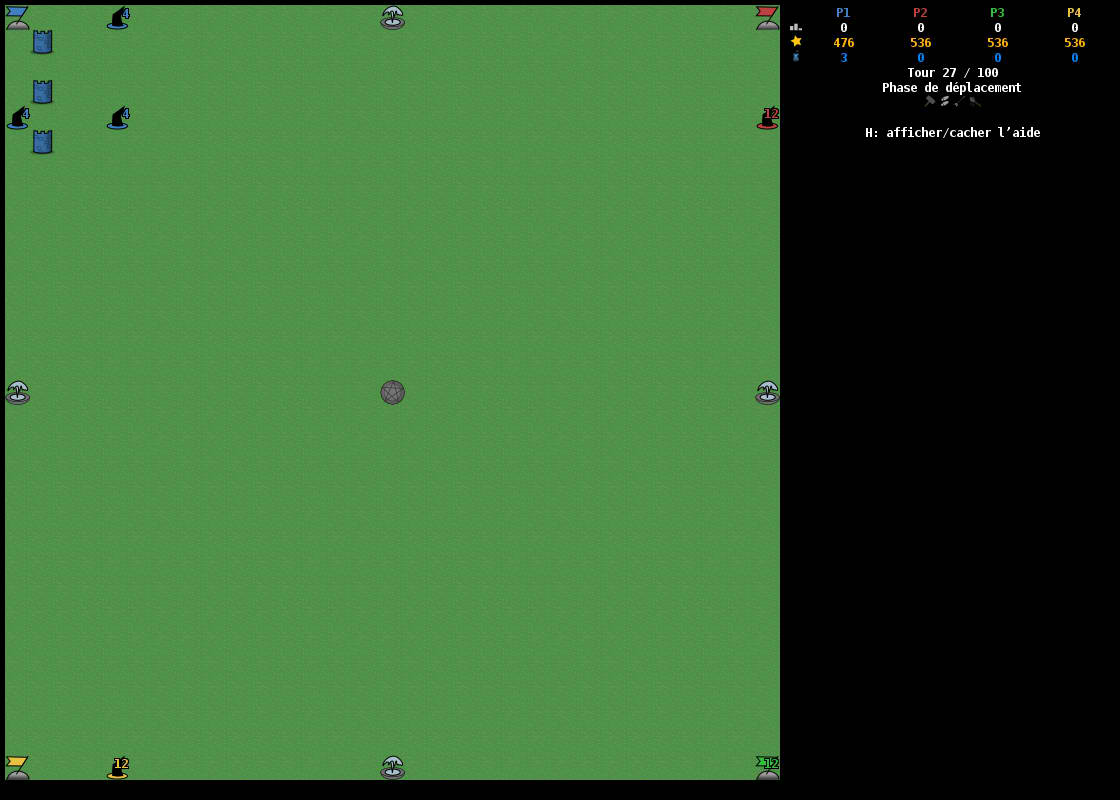
\includegraphics[width=\linewidth]{gui.jpg}
\end{frame}

\begin{frame}
	\frametitle{But du jeu}
	\begin{itemize}
	\item[1 pt] survivre à la fin de la partie
	\item[1 pt] conquérir le camp d'un joueur ennemi
	\item[1 pt] contrôler une fontaine de magie à la fin de la partie
	\item[4 pts] contrôler l'artefact à la fin de la partie
	\end{itemize}
\end{frame}

\begin{frame}
	\frametitle{Magie}
	\begin{itemize}
	\item[+] commencer un tour
	\item[+] contrôler une fontaine
	\item[+] détruire un sorcier adverse
	\item[\alert{--}] construire une tourelle
	\item[\alert{--}] produire un sorcier
	\end{itemize}
\end{frame}

\begin{frame}
	\frametitle{Quatre phases}
	\begin{itemize}
	\item[1] Construction
	\item[2] Déplacement
	\item[3] Tir des tourelles
	\item[4] Siège
	\end{itemize}
\end{frame}

\begin{frame}
	\frametitle{Construction}
	\begin{itemize}
	\item Les sorciers sont construits dans la base du joueur.
	\item Une tourelle doit être à 3 cases d'une autre tourelle (ou de la base) du même joueur
	\item … et même plus proche d'une tourelle du même joueur que de n'importe quelle tourelle d'un joueur ennemi.
	\item Un joueur peut détruire ses tourelles, mais cela ne lui rapporte aucun point de magie.
	\end{itemize}
	\pause
	\begin{itemize}
	\item \alert{20} points de magie pour construire une tourelle de portée \alert3
	\item 24 + 1 = \alert{25} points de magie $\Rightarrow$ tourelle de portée \alert4
	\item 24 + 4 = \alert{28} points de magie $\Rightarrow$ tourelle de portée \alert5
	\item 24 + 9 = \alert{33} points de magie $\Rightarrow$ tourelle de portée \alert6
	\end{itemize}
\end{frame}

\begin{frame}
	\frametitle{Déplacement}
	\begin{itemize}
	\item Les sorciers se déplacent par blocs.
	\item Les sorciers ne peuvent se déplacer sur les tourelles.
	\item Après déplacement, si des sorciers ennemis sont sur la même case, ils s'entretuent : le 2e plus grand nombre est retranché à tous les groupes.
	\end{itemize}
	\begin{example}[Exemple]
	\begin{itemize}
	\item 1 3 3 7 $\Rightarrow$ 0 0 0 4 et le 4\ieme{} remporte $1 + 3 + 3 = \alert7$ points.
	\item 4 2 4 2 $\Rightarrow$ 0 0 0 0
	\end{itemize}
	\end{example}
\end{frame}

\begin{frame}
	\frametitle{Tir des tourelles}
	\begin{itemize}
	\item Les tourelles répartissent leurs points d'attaque sur un ensemble de cases.
	\item 1 point d'attaque = 1 sorcier
	\item Les tourelles ne peuvent attaquer d'autres tourelles.
	\item Détruire un sorcier à distance ne rapporte pas de magie.
	\end{itemize}
\end{frame}

\begin{frame}
	\frametitle{Siège}
	\begin{itemize}
	\item Les sorciers peuvent attaquer les tourelles sur une case adjacente ($\uparrow$ $\uparrow$ $\downarrow$ $\downarrow$ $\leftarrow$ $\rightarrow$ $\leftarrow$ $\rightarrow$ B A)
	\item 1 sorcier = 1 point de vie en moins
	\item Une tourelle ne regagne pas de point de vie.
	\item À épuisement, la tourelle est détruite.
	\end{itemize}
\end{frame}

\begin{frame}
	\frametitle{Capture}
	\begin{itemize}
	\item Si un sorcier atteint la base d'un ennemi, ce dernier est anéanti (tourelles + sorciers).
	\item Si un sorcier se trouve sur une fontaine, il fait gagner des points de magie au joueur qui le contrôle.
	\end{itemize}
\end{frame}

\end{document}